\documentclass{article}
\usepackage[margin=1in]{geometry}
\usepackage{amsmath,amssymb}
\usepackage{verbatim}
\usepackage{graphicx}
\usepackage{xcolor,colortbl}
\usepackage[]{algorithm2e}
\usepackage{cite}
\usepackage{caption}
\usepackage{mdframed}

%\usepackage{soul}

\newcommand{\tab}{\hspace{10mm}}
\newcommand{\dtab}{\hspace{20mm}}
\newcommand{\ttab}{\hspace{30mm}}
\newcommand{\qtab}{\hspace{40mm}}

\begin{document}

\title{Autonomous Agents 1 \\ Assignment 2}

\author{By Group 4: Gieske, Gornishka, Koster, Loor}
\maketitle

\tableofcontents


\pagebreak

\section{Introduction}
This report contains the analysis of an implementation of single agent reinforcement learning. In these algorithms, the agent has no prior knowledge of the transition or reward function. Two different solutions to this problem are presented: in model-based learning, the agent learns the model from experience and plans on the learned model. In model-free learning, the agent learns state-values or Q-values directly. In this paper, model-free learning methods are considered.\\
Some prominent model-free reinforcement learning methods are on- and off-policy Monte Carlo Control, Q-learning (off-policy) and Sarsa (on-policy), where on-policy methods evaluate the values of a policy $\pi$ \textit{as it's being followed}, while off-policy methods allow the agent to follow a different policy $\pi'$. This paper reports on Q-learning and its on-policy equivalent, Sarsa. Moreover, the difference in action-selection between $\epsilon$-greedy and softmax are compared. 
\pagebreak

\section{Theory}
\subsection{Temporal difference learning methods}
Temporal difference learning methods estimate state-values or Q-values by updating them on every time step (as opposed to the episodic updates of Monte Carlo-methods).
Temporal difference learning methods are similar to Monte Carlo methods in that they both learn from experience directly, without requiring a model (thus, they do not exploit the Bellman-equations in equations \ref{eq:bellmanV} and \ref{eq:bellmanQ}) and they are similar to dynamic programming methods in that they both \textit{bootstrap}, i.e. they estimate values based on earlier estimates. 
\begin{mdframed}
\begin{align}
V^*(s) &= \sum_{s'} \mathcal{P}^a_{ss'}\left[ \mathcal{R}^a_{ss'} + \gamma \underset{a}{\text{max}}V^*(s') \right]\label{eq:bellmanV}\\
Q^*(s,a) &= \sum_{s'} \mathcal{P}^a_{ss'}\left[ \mathcal{R}^a_{ss'} + \gamma \underset{a}{\text{max}}Q^*(s', a') \right]\label{eq:bellmanQ}
\end{align}
\end{mdframed}

Thus, in general, an update-rule for a TD-method would be similar to that of TD(0) in equation \ref{eq:td0}.
\begin{mdframed}
\begin{align}
V(s) \leftarrow V(s) + \alpha [r+\gamma V(s') - V(s)]\label{eq:td0}
\end{align}
\end{mdframed}
Both Q-learning and Sarsa are TD-methods, and are described in more detail in sections Q-learning and Sarsa.

\subsection{Q-Learning} 
Q-learning is a temporal difference method that uses\footnote{More specifically, this is \textit{one-step Q-learning}, which is the algorithm evaluated in this paper.} the update rule in equation \ref{eq:qupdate}. Because it retrieves the Q-value of the state-action pair where Q(s', a) is maximized, it is an \textit{off-policy} method. The algorithm for Q-learning can be found in pseudocode in figure \ref{alg:qlearning}.

\begin{mdframed}
\begin{align}
Q(s_t, a_t) \leftarrow Q(s_t,a_t) + \alpha \left[ r_{t+1} + \gamma \underset{a}{\text{max}} Q(s_{t+1},a) - Q(s_t,a_t)\right]\label{eq:qupdate}
\end{align}
\end{mdframed}


\begin{center} 
\begin{mdframed}
\begin{algorithm}[H]
Initialize Q(s,a) arbitrarily \\
Repeat (for each episode):\\
\tab Initialize s \\
\tab Repeat (for each step of episode):\\
\dtab Choose a from s' using policy derived from Q (e.g., $\epsilon$-greedy)\\
\dtab Take action a, observe r, s'\\
\dtab Q(s,a) $\leftarrow$ Q(s,a) + $\alpha [ r + \gamma \max_a' Q(s', a') - Q(s, a) ]$  \\
\dtab s $\leftarrow$ s'; \\
\tab until s is terminal\\
\end{algorithm}
\end{mdframed}
\captionof{figure}{The algorithm for one-step Q-learning\cite{bartosutton}}
\label{alg:qlearning}
\end{center}



\subsection{Sarsa}
Sarsa is a temporal difference method that uses the update rule in equation \ref{eq:sarsaupdate}. Because it retrieves the Q-value of the state-action pair (s', a') where a' is selected using the policy $\pi$ that is being evaluated, it is an \textit{on-policy} method. The algorithm for Sarsa can be found in pseudocode in figure \ref{alg:sarsa}.
\begin{mdframed}
\begin{align}
Q(s_t, a_t) \leftarrow Q(s_t,a_t) + \alpha \left[ r_{t+1} + \gamma Q(s_{t+1},a_{t+1}) - Q(s_t,a_t)\right]\label{eq:sarsaupdate}
\end{align}
\end{mdframed}


\begin{center}
\begin{mdframed}
\begin{algorithm}[H]
Initialize Q(s,a) arbitrarily\\
Repeat (for each episode):\\
\tab Initialize s \\
\tab Choose a from s' using policy derived from Q (e.g., $\epsilon$-greedy)\\
\tab Repeat (for each step of episode):\\
\dtab Take action a, observe r, s'\\
\dtab Choose a' from s' using policy derived from Q (e.g., $\epsilon$-greedy)\\
\dtab Q(s,a) $\leftarrow$ Q(s,a) + $\alpha [ r + \gamma Q(s', a') - Q(s, a) ]$ \\
\dtab s $\leftarrow$ s'; \\
\tab until s is terminal\\
\end{algorithm}
\end{mdframed}
\captionof{figure}{The algorithm for Sarsa \cite{bartosutton}}
\label{alg:sarsa}
\end{center}



\subsection{Monte Carlo Methods}
As stated before, there are several ways of learning a estimating value functions and discovering optimal policies. Again, Monte Carlo methods do not know (nor need) complete knowledge of the environment. Monte Carlo methods require only experience, such as sample sequences of states, actions, and rewards, from on-line interaction with an environment. Unlike TD-methods, Monte Carlo methods require a model. The model only needs to generate sample transitions, unlike Dynamic Programming methods which need complete probability distributions of all possible transitions. Therefore, Monte Carlo methods are an important tool for an agent to use when only the model is known.

\subsection{On-policy Monte Carlo Control}
On-policy Monte Carlo control (ONMC) does not use exploring starts. In order to ensure that each state is visited and each action is selected infinitely often is to keep selecting these actions. There are two ways of implementing OPMCC; first-visit Monte Carlo and every-visit Monte Carlo. In this case, every-visit Monte Carlo is implemented which is reflected in the algorithm below. 

 
\begin{center}
\begin{mdframed}
\begin{algorithm}[H]
Initialize, for all $s \in \mathcal(S), a \in \mathcal(A)(s)$\\
\tab Q(s,a) $\leftarrow$ arbitrary \\
\tab Returns(s,a) $\leftarrow$ empty list \\
\tab $\pi \leftarrow$ an arbitrary $\epsilon$-soft policy \\
 
Repeat forever:\\
\tab Generate an episode using exploring starts and $\pi$\\
\tab For each pair s,a appearing in the episode:\\
\dtab $\mathcal{R} \leftarrow $ return following the first occurrence of s,a\\
\ttab Append $\mathcal{R}$ to $Returns(s,a)$\\
\ttab $Q(s,a) \leftarrow$ average($Returns(s,a)$)\\
\dtab For each $s$ in the episode:\\
\ttab $a^* \leftarrow$ arg $\max\limits_a Q(s,a)$\\
\ttab For all $a \in \mathcal{A}(s)$:\\

\qtab \[\pi(s,a) \leftarrow \left \{
\begin{array}{l l}
1-\epsilon + \dfrac{\epsilon}{|\mathcal{A}(s)|} & \quad \textit{if } a = a^* \\
\dfrac{\epsilon}{|\mathcal{A}(s)|} & \quad \textit{if } a \neq a^*
\end{array}\right.\]
\end{algorithm}
\end{mdframed}
\captionof{figure}{The algorithm for on-policy Monte Carlo \cite{bartosutton}}
\label{alg:OPMCC}
\end{center}


\subsection{Off-policy Monte Carlo Control}
Off-policy Monte Carlo control (OFFMC) does not use exploring starts. In order to ensure that each state is visited and each action is selected infinitely often is to keep selecting these actions. There are two ways of implementing OFMCC; first-visit Monte Carlo and every-visit Monte Carlo. In this case, every-visit Monte Carlo is implemented which is reflected in the algorithm below. 

 
\begin{center}
\begin{mdframed}
\begin{algorithm}[H]
Initialize, for all $s \in \mathcal{S}, a \in \mathcal{A}(s)$:\\
\tab Q(s,a) $\leftarrow$ arbitrary\\
\tab N(s,a) $\leftarrow$ 0; Numerator\\
\tab D(s,a) $\leftarrow$ 0; Denominator of Q(s,a)\\
\tab $\pi \leftarrow$ an arbitrary deterministic policy\\

Repeat forever:\\
\tab Select a policy $\pi '$ and use it to generate an episode:\\
\dtab $s_0, a_0, r_1, s_1, r_2, ..., s_{T-1}, a_{T-1}, r_T, s_T$ \\
\tab $\tau \leftarrow$ latest time at which $a_t \neq \pi (s_{\tau}, a_{\tau})$\\
\tab For each pair s, a appearing in the episode at time $\tau$ or later:\\
\dtab $\tau \leftarrow$ the time of first occurrence of s, a such that $t \leq \tau$\\
\dtab $w \leftarrow \prod\limits_{k=t+1}^{T-1} \dfrac{1}{\pi'(s_k, a_k)}$\\
\dtab N(s,a) $\leftarrow$ N(s,a) + $wR_t$\\
\dtab D(s,a) $\leftarrow$ D(s,a) + $w$ \\
\dtab Q(s,a) $\leftarrow \dfrac{N(s,a)}{D(s,a)}$ \\
\tab For each $s \in \mathcal{S}$: \\
\dtab $\pi(s) \leftarrow$ arg $\max_a$ Q(s,a)\\
\end{algorithm}
\end{mdframed}
\captionof{figure}{The algorithm for off-policy Monte Carlo \cite{bartosutton}}
\label{alg:OFFMC}
\end{center}



\subsection{Action selection methods}
In order to select which action to choose according to a given policy, a tradeoff between exploration and exploitation must take place. This tradeoff is important when performing reinforcement learning as the rewards must be maximized, but exploration may lead to finding higher rewards. There are several action selection methods which can be used to select actions. The two techniques analyzed in this report are $\epsilon$-greedy and softmax action selection.

In the case of $\epsilon$-greedy, the best action $a^*$ is given a probability of $1-\epsilon$. All actions $a$ (including $a^*$) then receive an equal portion of $\epsilon$ as a probability. This is formalized in equation \ref{eq:greedy}.
\begin{mdframed}
\begin{align}
\forall a \in \mathcal{A}:p(a) = 
\begin{cases}\label{eq:greedy}
	1 - \epsilon + \frac{\epsilon}{|\mathcal{A}|}, & \text{if } a = a^*\\
	\frac{\epsilon}{|\mathcal{A}|} & \text{otherwise }
\end{cases}
\end{align}
\end{mdframed}
So that in $1-\epsilon$ of the cases, $a^*$ is selected, and in $\epsilon$ of the cases a random action is chosen uniformly. Thus, an $\epsilon$-greedy policy mainly exploits the known states to maximize the immediate reward. At probabilistically determined times however, this policy will explore new states. This may lead to undesired behavior as it is possible for the agent to stand beside the goal state when the $\epsilon$-greedy policy turns to explore a new state, which can lead to high negative rewards in particular cases, such as a robot falling off a cliff. Also, $\epsilon$-greedy does not consider the quality of non-optimal actions: an action with a value just below that of $a^*$ receives the same probability as an action with a much lower value. Another note using $\epsilon$-greedy is the intuition that $\epsilon$ should decay as the agent has explored more states, as exploration is adding less information over time. There is, however, no clear-cut way to do decide how and when to decay $\epsilon$.

Softmax action-selection offers a solution to one problem presented by $\epsilon$-greedy policies. The greedy action $a^*$ is still assigned the highest probability, but all other probabilities are ranked and weighted according to their values [1]. There are several ways of implementing the softmax action selection method, but for the purposes of this paper softmax uses a Boltzmann distribution, formalized in \ref{eq:softmax}.
\begin{mdframed}
\begin{align}
\forall a: p_t(a) &= \frac{\text{e}^{Q_t(a)/\tau}}{\sum^n_{b=1}\text{e}^{Q_t(b)/\tau}} \label{eq:softmax}
\end{align}
\end{mdframed}
The parameter $\tau$ in equation $(2)$ is the \textit{temperature} of the distribution. Low temperatures cause the values of $Q_t(a)$, and consequently those of e$^{Q_t(a)/\tau}$, to grow much larger, thus increasing their differences. This leads to assigning a high probability to the optimal action and assigning lower probabilities to suboptimal actions. Of course, terrible actions get very low probabilities. For high temperatures, the opposite is true, where in the limit $\tau\rightarrow0$, all actions become equiprobable [1].

It is unclear whether $\epsilon$-greedy action selection is better than softmax action selection. The performance of either method may depend on the task at hand and human factors. Experimenting with both methods will lead to more insight in both algorithms.
\pagebreak

\section{Implementation}
The implementation consists of the following files:
\begin{description}
	\item[Agents\_new] \hfill \\ 
	This file contains implementions of the Agent class, the Prey class and the Predator class. Both the predator and the prey inherit functions of the Agent class. The Agent class contains functions any agent needs, such as a set of actions, a policy and other functions. As the predator is the agent is the agent this implementation focuses on, the predator class contains more functions than the predator class.
	
	\item[Helpers] \hfill \\ 
	This file contains many helper functions. These functions aid in computation and decision making, but cannot (and need not) be part of a specific class.
	
	\item[Other\_objects] \hfill \\ % uncertain about policy class description
	This file contains the Policy and Environment classes. The environment of the game as well as the rules are implemented in the Environment class. The Policy class contains the implementation of Q-Learning, Sarsa, $\epsilon$-greedy, softmax action selection and more functions that help in determining and optimizing a policy as well as choosing an action of this policy.
	\item[Newstate] \hfill \\ 
	This file contains the Game class as well as a demonstration function. The Game class instantiates the game, initialized the predator and the prey and assigns policies to these. The game is run N times and the result is printed. The demonstration function also performs Q-Learning, Sarsa and Monte Carlo. It also uses $\epsilon$-greedy and softmax action selection. The results are printed in the command line and graphs are used for analysis.
\end{description}
\pagebreak
\section{Analysis}
This section discusses the results of the implementations. In order to display and compare results, graphs are used. The title describes which parameters are analysed and the legend shows which color represents which setting of said parameters.

\subsection{Q-Learning}

\subsubsection{Different discount factors}
First, the effects of different discount factors on Q-learning is analysed. The results are displayed in the figure below.

\begin{center}
	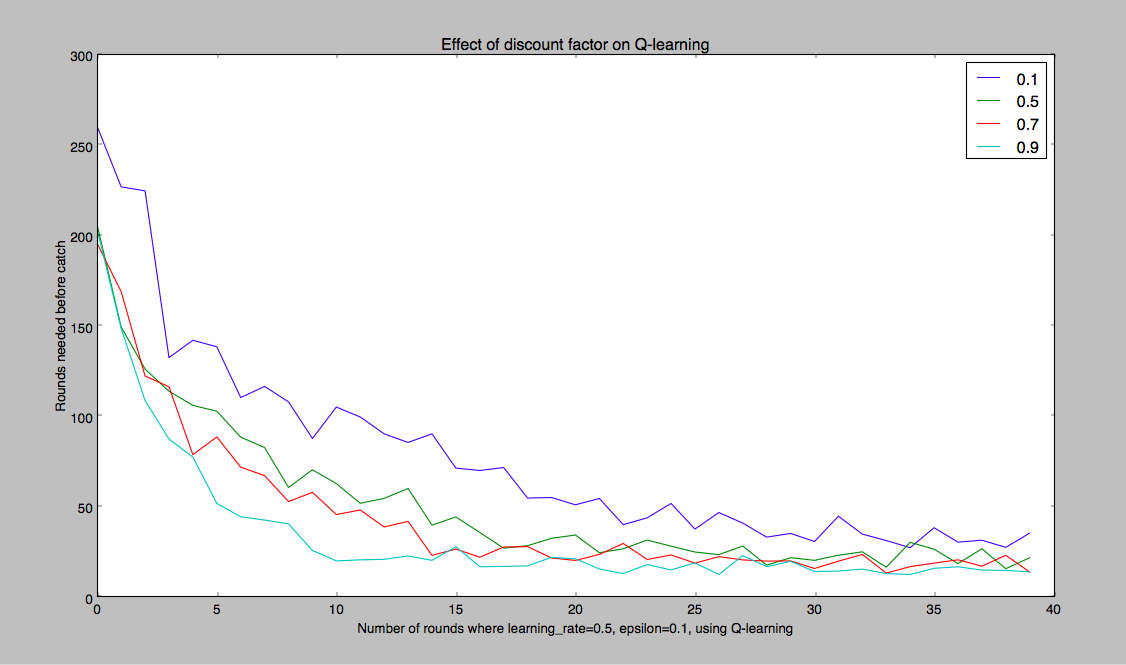
\includegraphics[scale=0.4]{discount_factors}
	\captionof{figure}{Q-learning using different discount factors}
\end{center}

%\begin{figure}[h!]
%\begin{center}
%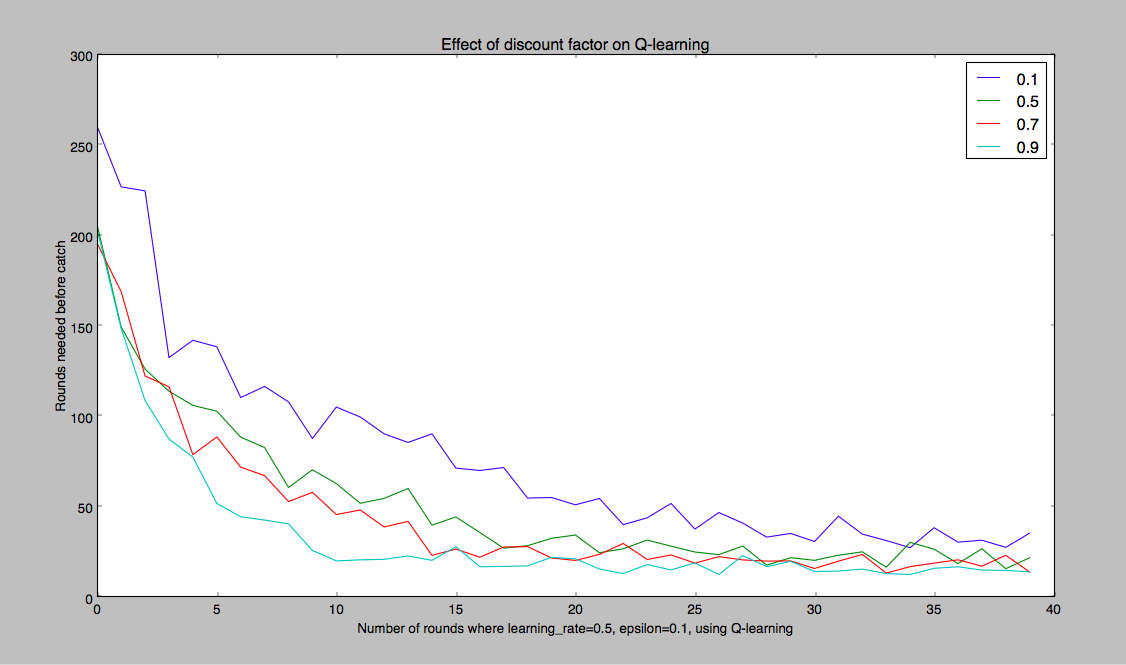
\includegraphics[scale=0.4]{discount_factors}
%\caption{Q-learning using different discount factors}
%\end{center}
%\end{figure}

As shown, the higher the discount factor, the better the result. The height of the discount factor determines the importance of future rewards. A low discount rate tries to achieve a high immediate reward and a high discount rate tries to achieve a high overall reward. Since reaching each state yields a reward of 0, except for the goal state which yields a reward of 10, the future reward must be maximized. Therefore, this behaviour can be expected. 

\subsubsection{The effect of $\epsilon$}
As Q-learning is a learning algorithm, exploration and exploitation must be balanced well to find the optimal behaviour. The following graph shows different settings for $\epsilon$. 

\begin{center}
	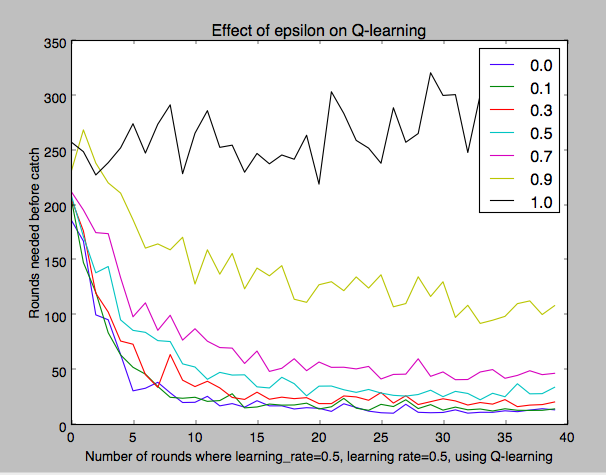
\includegraphics[scale=0.4]{epsilons}
	\captionof{figure}{Q-learning using different epsilon values}
\end{center}

As shown in the figure above, the lower the $\epsilon$ value is, the quicker the algorithm finds the optimal path. This can be expected since, as stated in the theory, an $\epsilon$ value of 0 leads to a greedy algorithm. What is interesting is that an $\epsilon$ value of 0.9 performs quite well compared to a completely exploratory policy, which seems to lead to random results. This shows how important explorations is and how strong an $\epsilon$-greedy policy is. Even with the slightest bit of greedy behaviour, good results are achieved.

\subsubsection{Different learning rates}
It is possible to set different learning rates in Q-learning. The learning rate determines to which extent the new information will overwrite the old information. The following graph shows how important the relationship of old and new information is to achieve an optimal policy.

\begin{center}
	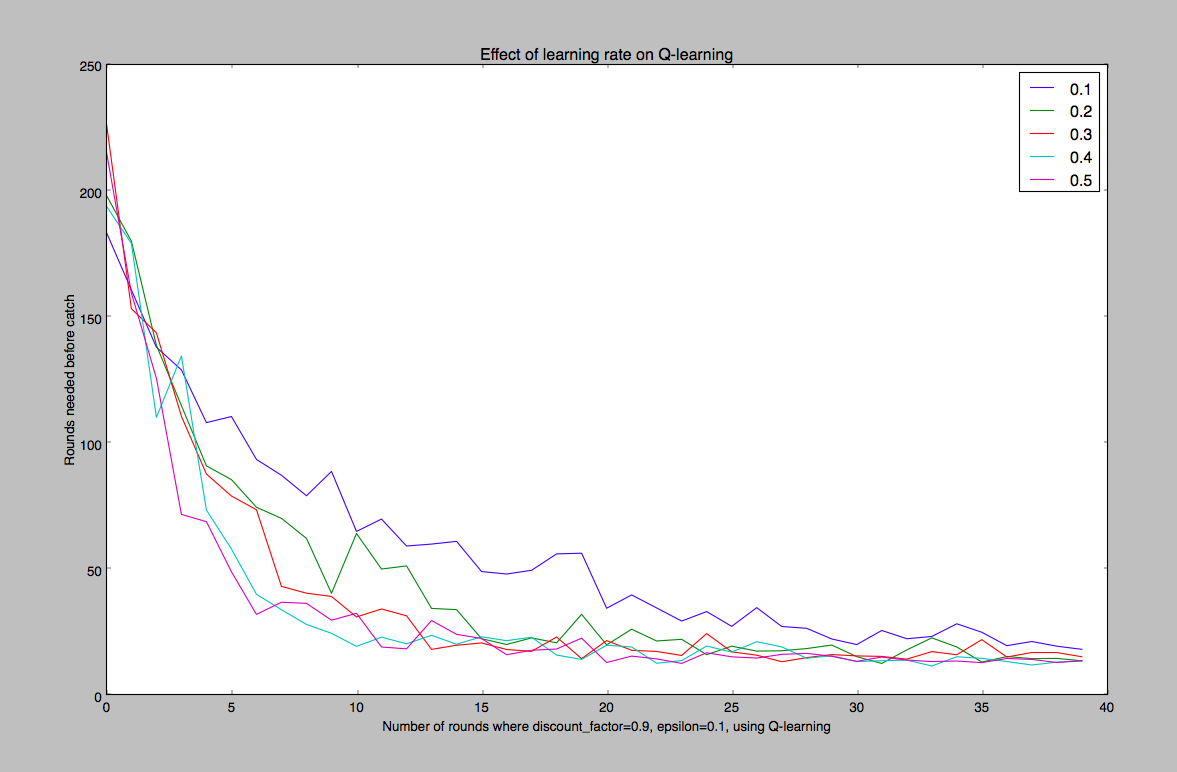
\includegraphics[scale=0.4]{learning_rates}
	\captionof{figure}{Q-learning using different learning rates}
\end{center}

%\begin{figure}[h]
%\begin{center}

%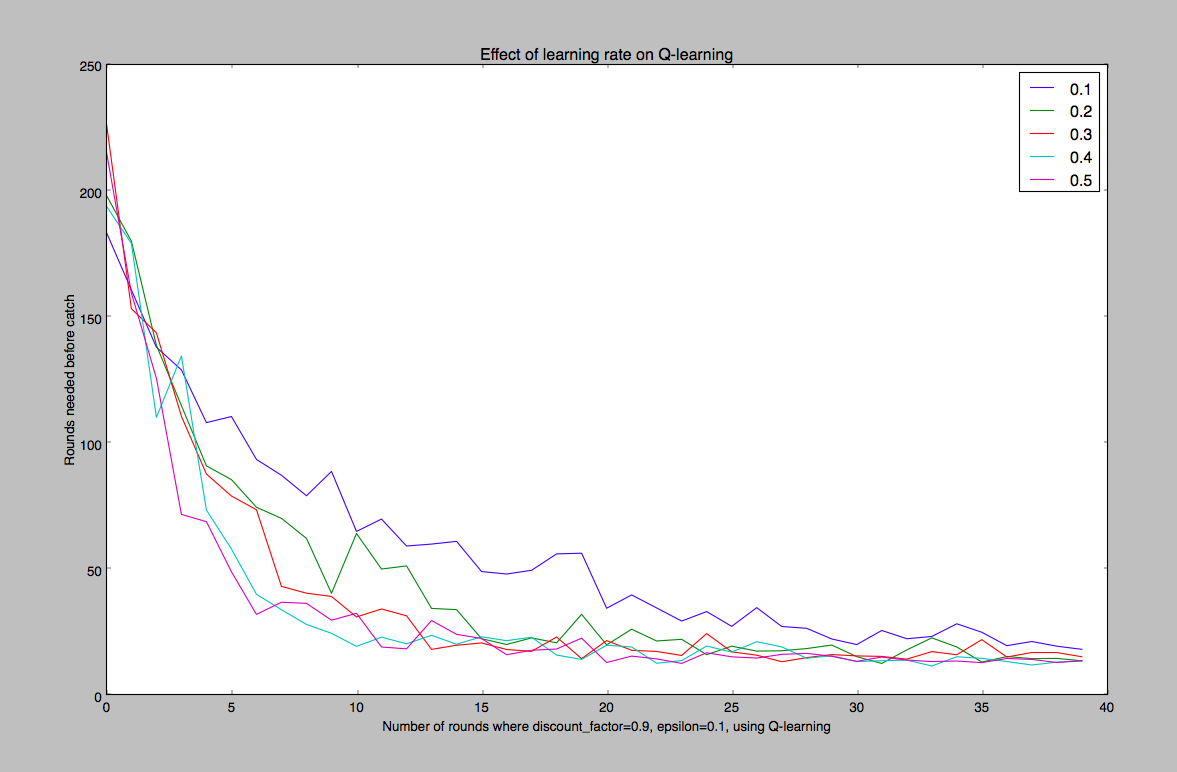
\includegraphics[scale=0.4]{learning_rates}
%\caption{Q-learning using different learning rates}
%\end{center}
%\end{figure}

The figure above shows that for each learning rate between, and including, 0.1 and 0.5 leads to conversion. However, a low conversion rate leads to slower conversion than a high conversion rate. It is interesting to note that the learning rates of both 0.4 and 0.5 appear to converge at about the same speed. Remember that the learning rate determines to which extent the new information will overwrite the old information. It appears that, even when storing little new data, this leads to convergence. The more new data overwrites the old data the quicker the algorithm converges. Intuitively, this seems to be correct. However, overwriting all old data might lead to less than optimal behaviour. As stated before, learning rates of 0.4 and 0.5 seem to yield the same result. It is well possible that this is the limit until which the learning rate factor is beneficial to the algorithm. As this lies beyond the scope of this report, this can be researched in the future.

\subsubsection{Different initialization for Q-learning}
It was advised to initialize the policy of the predator optimistically, when performing Q-learning. When initializing a policy optimistically, it is interesting to see what happens when a policy is not optimistically initialized. The values chosen are 15, 10, 5, 0 and -5. Also, to see the effect of learning, the $\epsilon$-value was set to either 0 or 0.1. The figure below shows the results of $\epsilon$ value 0.1.

\begin{center}
	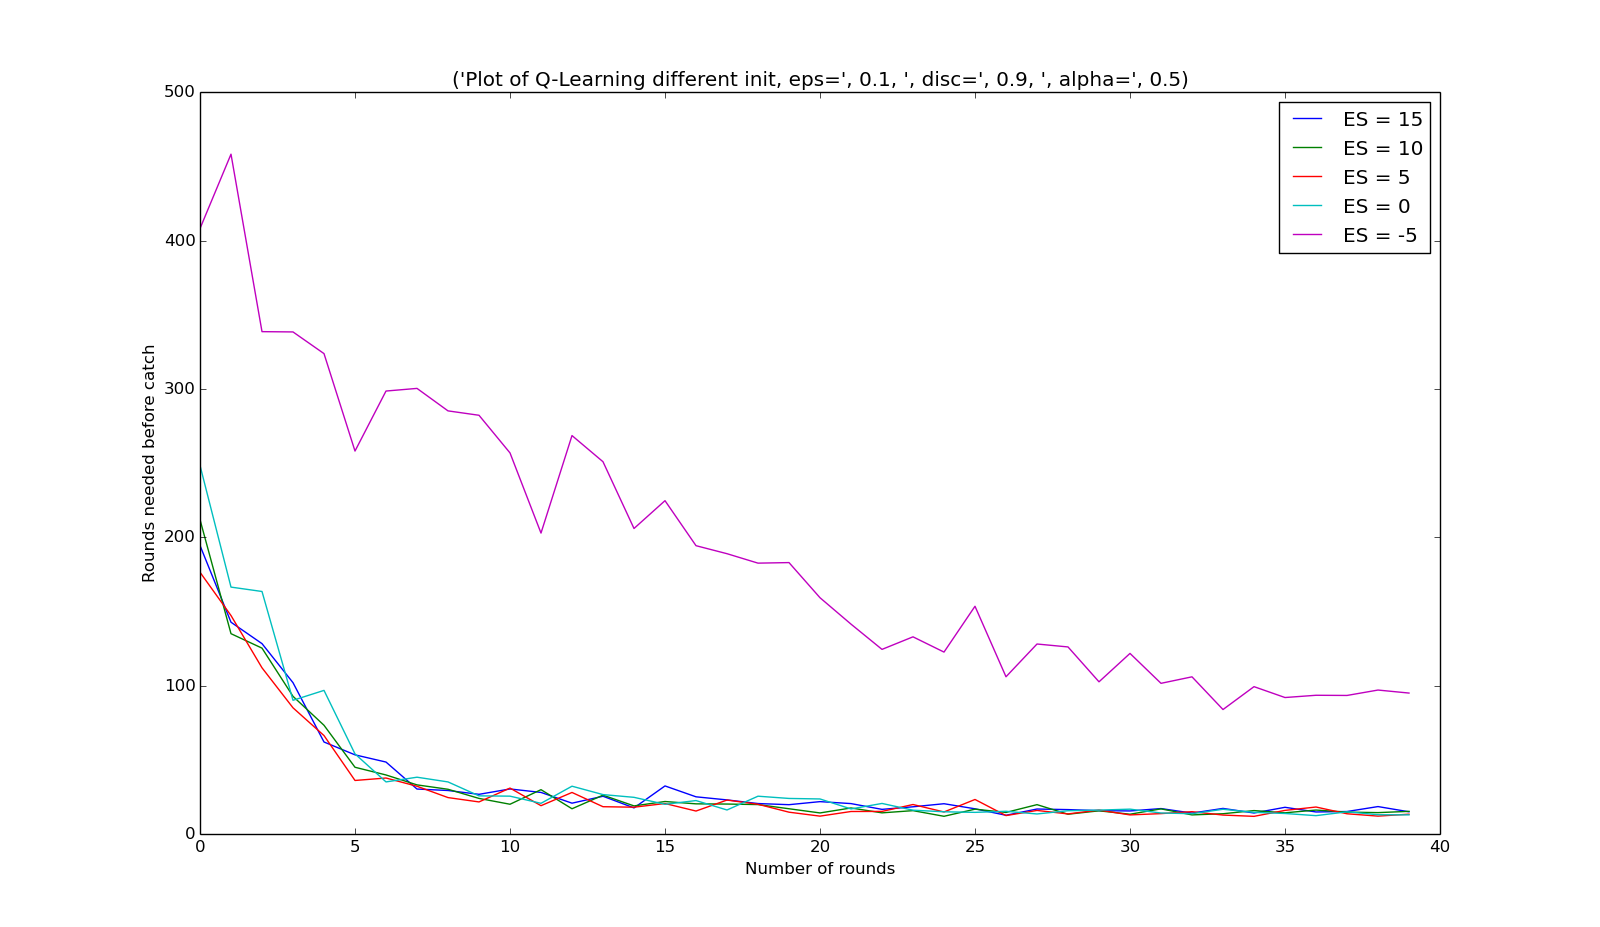
\includegraphics[scale=0.4]{q_learnin_diff_init_epsilon_0_1}
	\captionof{figure}{Q-learning with different policy initialization values and $\epsilon$ is 0.1}
\end{center}

Each non-negative initialization appears to yield good results. Though it takes an initialization of 0 longer to converge, the policy does eventually converge to the same level as the optimistic policy. The negatively initialized policy behaves very poor. It does improve, but it takes significantly longer to converge than the non-negative initialized policies. It is expected that both the negative and zero initialization lead to slow learning. However, it is possible that the zero initialization is a border case where this is (one of) the last case(s) where the algorithm still learns enough to perform well.

%\begin{figure}[h]
%\begin{center}
%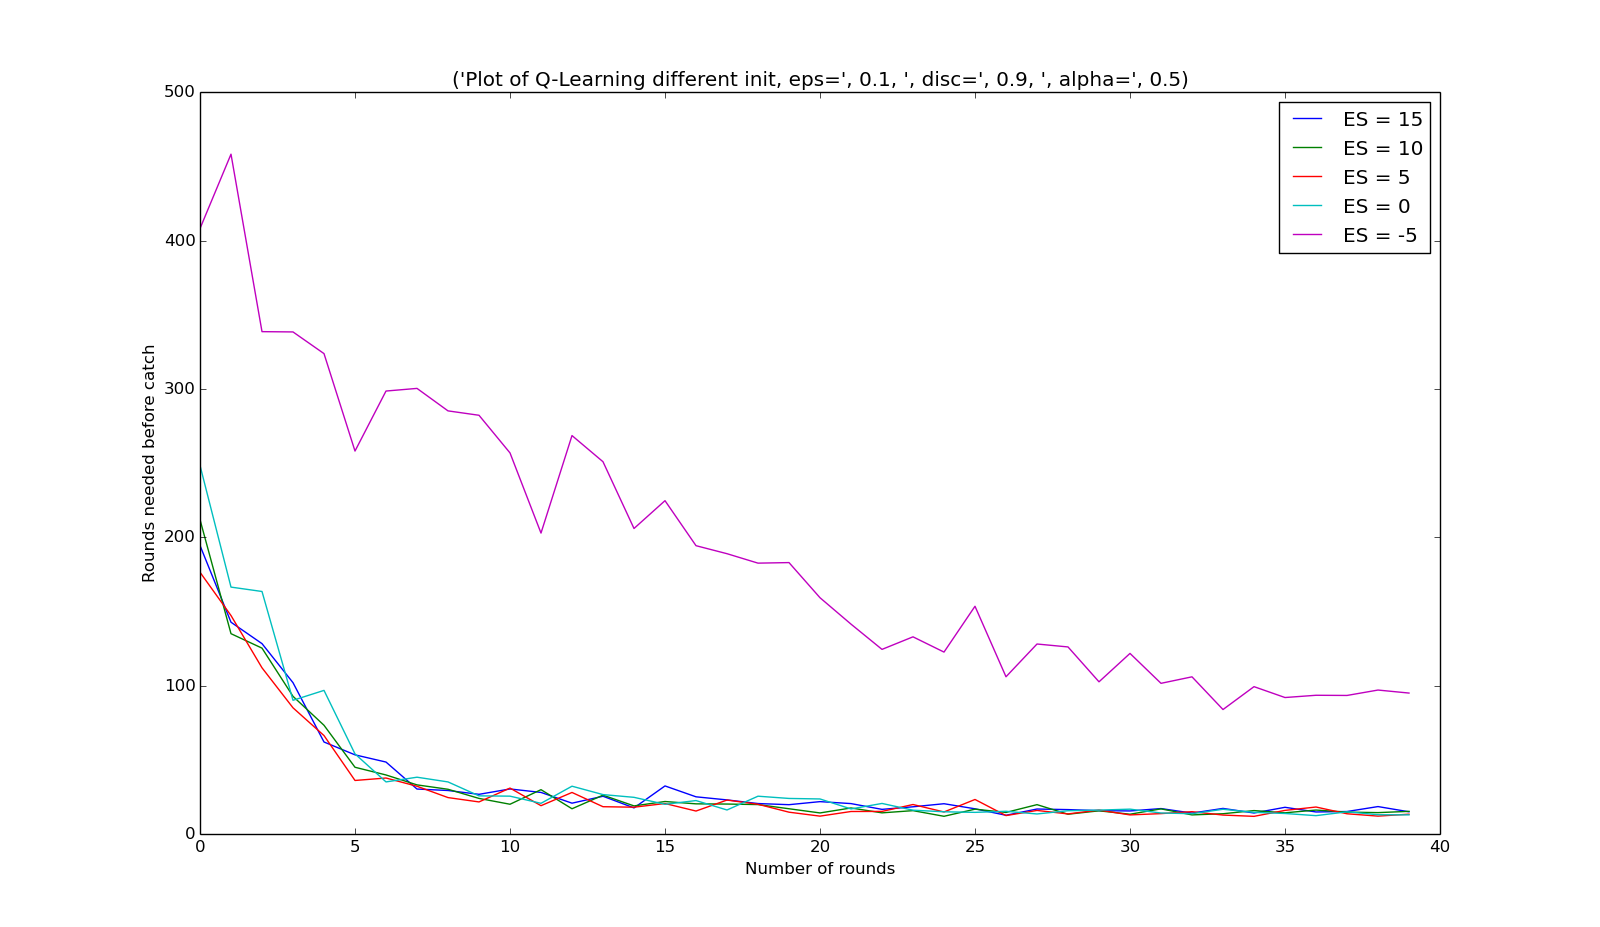
\includegraphics[scale=0.4]{q_learnin_diff_init_epsilon_0_1}
%\caption{Q-learning with different initialization values and $\epsilon$ is 0.1}
%\end{center}
%\end{figure}

Now let's analyse the same initialization values with an $\epsilon$-value of 0.
\begin{center}
	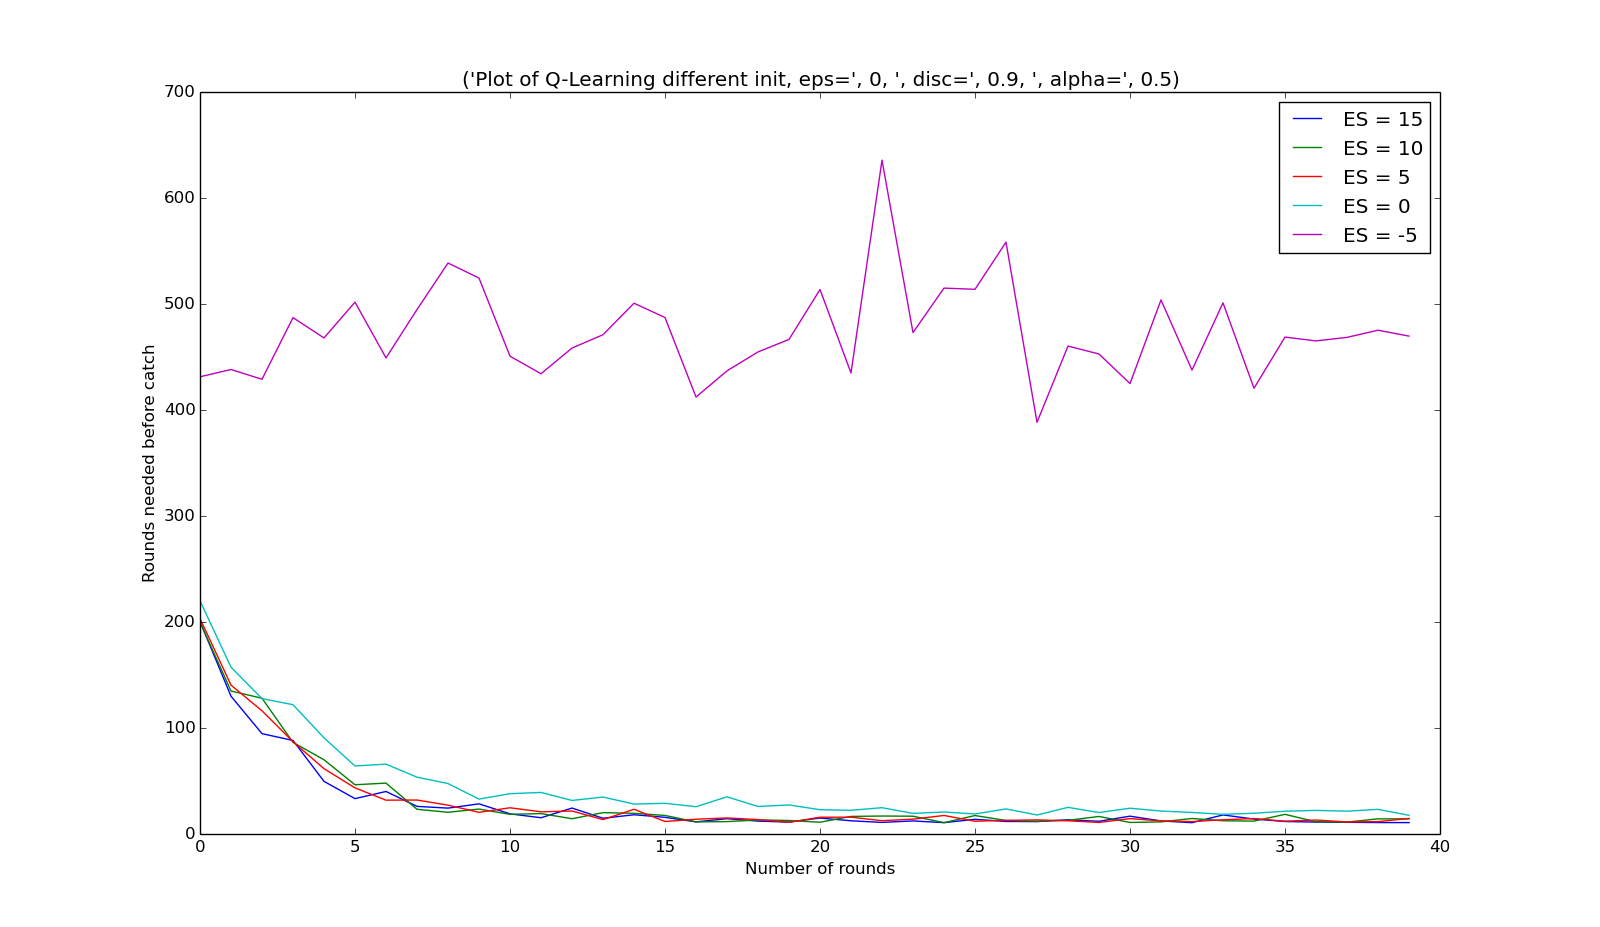
\includegraphics[scale=0.4]{q_learning_diff_init_epsilon_0}
	\captionof{figure}{Q-learning with different initialization values and $\epsilon$ is 0}
\end{center}
This leads to similar results as before. One of the differences is that the policy initialized with 0 performs worse than before and does not converge. This behaviour can be expected. At the non-negative initializations, there are values larger than zero. Therefore, executing a greedy policy still leads to convergence. As stated, it is expected that the initialization with zero values should behave similar to the negative initialization. Again, this is not the case. This is still a border case, as stated before.

In order to determine whether the zero initialization is indeed a border case, more runs can be performed. However, this falls beyond the scope of this report. It is important to test this is the future to determine the limits of this implementation.
%\begin{figure}[h]
%\begin{center}
%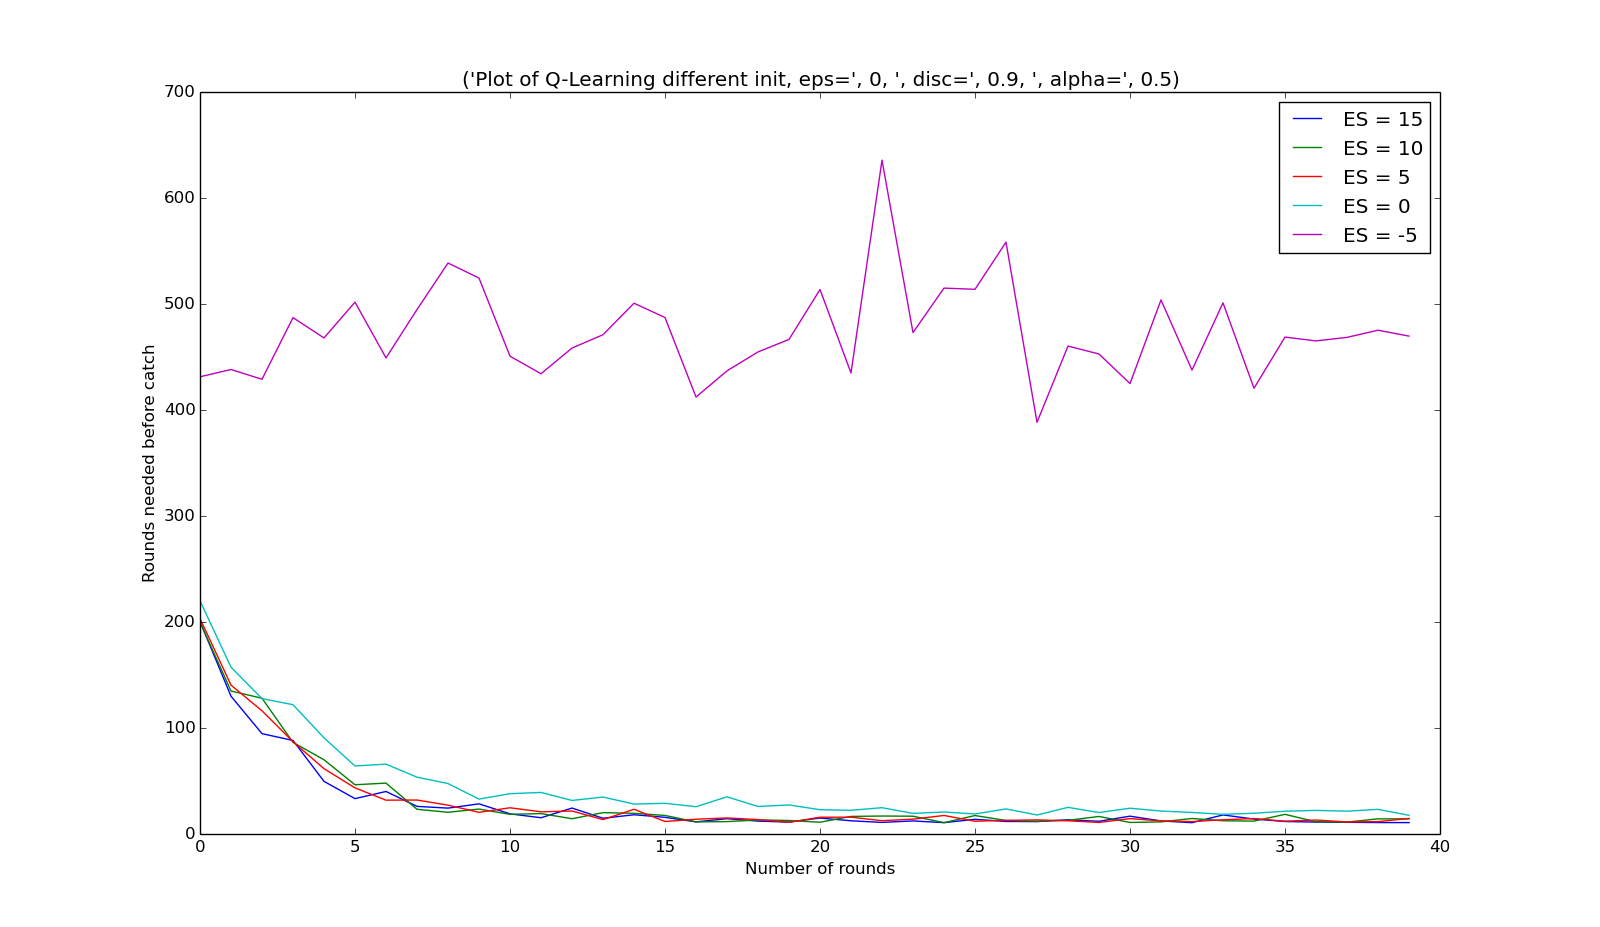
\includegraphics[scale=0.4]{q_learning_diff_init_epsilon_0}
%\caption{Q-learning with different initialization values and $\epsilon$ is 0}
%\end{center}
%\end{figure}

\subsubsection{$\epsilon$-greedy vs. softmax}
As the effect of $\epsilon$-greedy action selection on Q-learning has already been discussed, let's analyse the effect of softmax action value selection. 
% Explain that smaller grid takes longer to converge, since the predator is more likely to catch the prey, so it takes more rounds to actually explore enough. On the other hand, in a bigger grid the predator is highly unlikely to catch the prey, so it would explore a lot even in one round by the time it catches the prey.

\begin{center}
	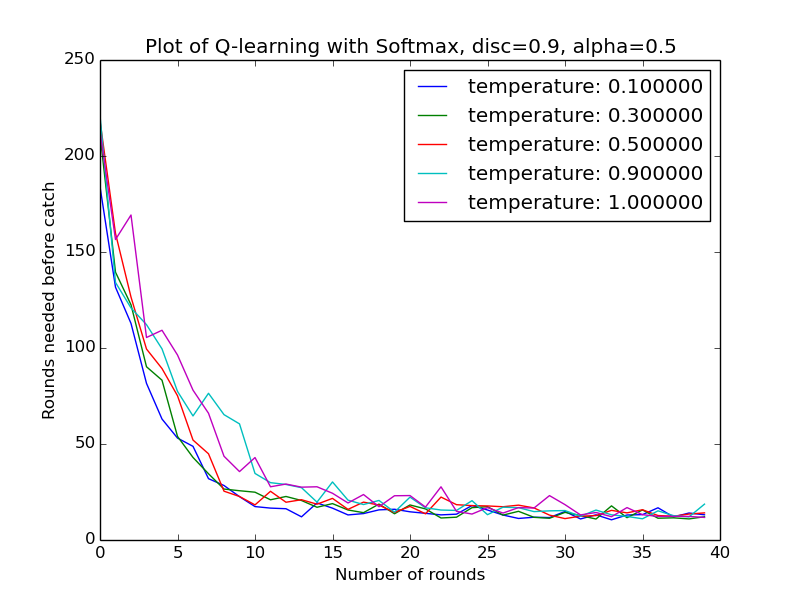
\includegraphics[scale=0.4]{softmax_with_legend}
	\captionof{figure}{Q-learning using different temperatures in Soft-max}
\end{center}

The graph shows that all results converge. It shows that the lower the temperature, the better the results. This is to be expected, as the lower the temperature leads to a greedy action selection. However, the temperature of the softmax action selection algorithm can not be zero, as the temperature is divided by. This ensures both optimal action selection and exploration. When analysing the higher temperatures, it these converge at about the same speed as the low temperatures. However, the higher the temperature, the less smooth the graph. As a high temperature (e.g. $\tau$ is 1) leads to an equiprobable action selection, the algoritm both explores and exploits to a certain level. This causes the algorithm to converge, but also taking longer (compared to lower temperatures such as $\tau$ is 0.1) to catch the prey in an episode.

Now let's look at the results between softmax and $\epsilon$-greedy. As stated in the theory, the difference in effect between softmax action selection and $\epsilon$-greedy action selection is unknown. The performance of either relies on the goal of the implementation, as well as human factors. Therefore, it is imperative to research the effects on this implementation. The $\epsilon$ value chosen for the $\epsilon$-greedy algorithm is the same as the temperature, $\tau$. This means that both algorithms behave greedy, but still explore from time to time.

\begin{center}
	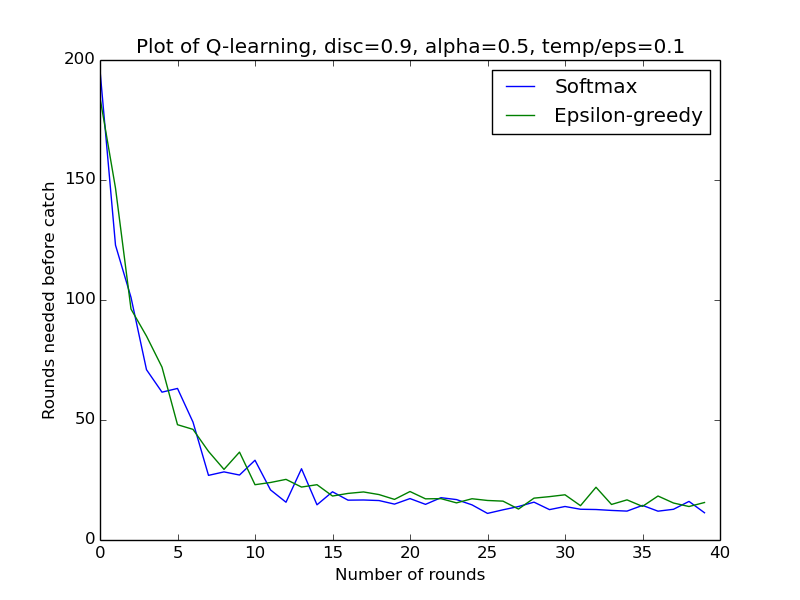
\includegraphics[scale=0.4]{softmax_vs_egreedy}
	\captionof{figure}{Q-learning $\epsilon$-greedy and softmax action selection}
\end{center}

The figure shows that both softmax and $\epsilon$-greedy action selection converge at the same speed. However, softmax action selection eventually leads to capturing the prey in less rounds. Therefore, softmax action selection is preferred over epsilon-greedy action selection when the the prey needs to be caught in a minimum amount of timesteps.

\subsection{Learning types}
Aside from Q-learning, Sarsa and on-policy Monte Carlo were implemented. It is interesting to see the difference in performance between the algorithms. The results are shown in the figure below.

\begin{center}
	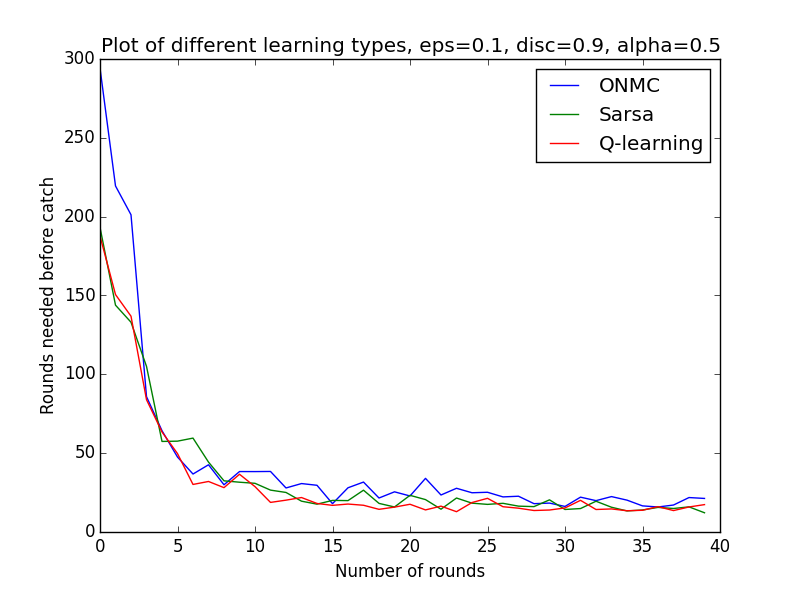
\includegraphics[scale=0.4]{learning_types}
	\captionof{figure}{Different learning types set out against one another}
\end{center}

The figure shows that all algorithms converge. Q-learning converges quickest, with Sarsa not much slower. On-policy Monte Carlo also converges quickly, but it starts with the worst Q-values. It also shows that of all algorithms, on-policy Monte Carlo converges to the least optimal number of rounds that lead to convergence. %yeah, not sure... at all!!
% CHECK THIS AS I AM REALLY NOT CERTAIN!

The following table shows how many rounds were needed, per learning type on average, for the prey to catch the predator. This was calculated for the first 1000 runs  and the last 1000 runs. This means that the learning in the very beginning and the learning in the very end are set out against each other.

\begin{tabular}{| l | l | l | l | l |}
\hline
 & \parbox{2cm}{\textbf{Avg nr/rounds\\ (first 1000)}} & \parbox{2cm}{\textbf{Avg nr/rounds\\ (last 1000)}} & \parbox{2cm}{\textbf{STD\\ (first 1000)}} & \parbox{2cm}{\textbf{STD\\ (last 1000)}} \\
\hline
\textbf{Q-learning} & 88.68 & 14.52 & 124.39 & 18.84 \\
\hline
\textbf{Sarsa} & 80.61 & 14.70 & 109.74 & 22.45 \\
\hline
\textbf{ONMC} & 79.68 & 15.78 & 112.11 & 21.64 \\
\hline
\end{tabular}

\section{Conclusion}
Q-learning is an effective method to learn the Q-values of the states of environments. This leads to learning about the states of an environment and planning to take the optimal action. Several parameters need to be tuned to achieve optimal performance. These parameters are the learning rate  ($\alpha$), the discount factor ($gamma$), the action selection method, $\epsilon$, $\tau$ and the behavioural initialization. 

\subsection{Discount factor}
The effects of the discount factor on Q-learning shows that a high discount factor leads to best results. This makes the future rewards more important. As stated in the analysis, this is expected as the reward for all stated, but the goal state, is 0. The reward of the goal state is 10, at which the episode ends. This leads to a very important future reward that must be maximized.

\subsection{Learning rates}
Different learning rates determine how important old information is. The higher the learning rate, the more new information overwrites the old information. As the effects of learning rates of 0.1 to 0.5 are tested, it is clear that the height of the learning rate affects the convergence speed. However, it appears that a learning rate of 0.4 and 0.5 perform almost equally well. This could be the tipping point of the effect of the learning rate. It is very well possible that a learning rate higher than 0.5 leads to worse results. This occurs due to the tradeoff between the learning speed and learning wrong behaviour. It is possible the goal state was reached due to luck. This means that the optimal behaviour, determined with a learning rate higher than 0.5, can be based on coincidence. 

\subsection{Action selection methods}
When choosing an action selection method, two of the most common methods are $\epsilon$-greedy action selection and softmax action selection. As the optimal tradeoff between exploration and exploitation is difficult to balance, these algorithms can be tested and the best performing algorithm with the best settings can be chosen. In order to determine how important these algorithms are, both were tested with Q-learning. Also, a relatively greedy policy was tested in both cases and compared to one another. 

\subsubsection{$\epsilon$-greedy action selection}
When using the $\epsilon$-greedy action selection, an $\epsilon$ value of 1 leads to a completely exploratory behaviour. This does not lead to convergence. Any $\epsilon$ value lower than 1 leads to convergence. The lower the $\epsilon$ value, the quicker convergence is achieved. Also, the lower the $\epsilon$ value, the less timesteps the predator needs to capture the prey. This is caused by the fact that an $\epsilon$ value of 0 leads to a greedy policy.	As the environment is fairly static, the predator does not need to learn much to at least get near the prey. In addition, the optimal grid initialization leads to quite radical changes in Q-values. Meaning, if a visited state is not optimal, the Q-value of that state will drop significantly. On the other hand, optimal states will maintain a high value. 

\subsubsection{Softmax action selection}
Softmax action selection shows that the lower the temperature, the quicker and better Q-learning converges. This is to be expected as the lower the temperature, the more greedy the action selection algorithm behaves. The difference between $\epsilon$-greedy and softmax is that softmax cannot become explicitly greedy. The algorithm will always explore, as the temperature cannot become 0. In the algorithm, this will lead to dividing by 0 and this is impossible. 

\subsubsection{Softmax vs. $\epsilon$-greedy}
When setting out $\epsilon$-greedy action selection against softmax action selection, it appears that both perform well. Both converge at similar speeds, but softmax action selection makes the predator catch the prey in less timesteps.

\subsubsection{Varying grid initialization}
As the grid was initialized optimistically, it is interesting to see what happens when the grid is not optimistically initialized. The grid was initialized with the values 15, 10, 5, 0 and -5. This way, changes while lowering the grid initialization will become clear. In order to research what happens with different $\epsilon$ values, this was tested with $\epsilon$ values of 0 and 0.1. 

In the case of $\epsilon$ is 0.1, all initializations lead to convergence. However, the negative initialization lead to very slow convergence. In this case, it is expected for the grid initialization of 0 to behave similarly to the negative initialization. This, because the Q-value is 0 and therefore already is very low. This is not the case and leads to the conclusion that the grid initialization with 0 leads to a border case, where this is (one of) the smallest value(s) for the algorithm to converge.

In the case of $\epsilon$ is 0, again all non-negative initialized grids lead to convergence. The grid initialized with zeros does converge slowest and has the lowest convergence values (in other words, it takes longest for the predator to catch the prey). The negative initialized grid does not converge. This can be attributed to the fact that the policy is explicitly greedy. In this case, that leads to following a path that does not improve over time and no learning. 


\subsubsection{Learning types}
%This conclusion is probably incorrect as the analysis is incomplete!
After analysing the results, it can be concluded that the use of both Monte Carlo methods as well as temporal difference methods converge quickly. However, temporal difference methods outperform on-policy Monte Carlo. Of the temporal difference methods, Q-learning outperforms Sarsa as well. The differences are minimal, but they are there. Nevertheless, both converge to almost the same result. This leads to the conclusion that either Sarsa or Q-learning can be implemented, whatever the requirements, and the same results can be expected.

\section{Future work}
In the report some results lead to more questions or needed more research than was conducted. Some of these questions were already mentioned in the report and are repeated here. 
Encoded version
learning rate > 0.5

\section{Files attached}
\begin{itemize}
\item newstate.py
\item agents\_new.py
\item other\_objects.py
\item helpers.py \ldots
\end{itemize}

\section{Sources}

\bibliography{bibliography}
\bibliographystyle{plain}
\begin{itemize}
	\item [1] Barto and Sutton (http://webdocs.cs.ualberta.ca/~sutton/book/the-book.html) \ldots
\end{itemize}

\end{document}
